%% %% %% %%
%%
%% Parte C de la práctica
%%
%% %% %% %%

\documentclass[../procedimientos.tex]{subfiles}
\graphicspath{{\subfix{../../images/}}}

\begin{document}
\clearpage
\subsection{Parte C}
\subsubsection{Propuesta}
Luis, Ana y sus padres van al cine bajo ciertas condiciones que son limitadas 
por la Madre y el Padre. Ellos van al cine si la Madre y el Padre están 
totalmente de acuerdo, si los dos no lo están, entonces no pueden ir. Ahora, 
si los dos están en desacuerdo, la salida al cine debe ser resuelta por 
mayoría absoluta entre todos los integrantes de la familia. Si existe un 
empate general, la decisión será tomada por la madre. Diseñar un circuito 
digital que señalice con un diodo LED el momento cuando pueden ir al cine.

\subsubsection{Análisis}
De forma general, el sistema tiene cuatro entradas: $l$, $a$, $m$ Y $p$ (el 
voto de Luis, Ana, su Madre y su Padre respectivamente); y la salida estará 
dada por el valor de $c(lamp)$.  La Implementación de la tabla de verdad del 
problema se muestra a continuación:
\begin{table}[H]
  \centering
  \begin{tabular}{cccc|ccc}
    \hline
    $l$ & $a$ & $m$ & $p$ & $c$\\
    \hline
    0 & 0 & 0 & 0 & 0\\
    0 & 0 & 0 & 1 & 0\\
    0 & 0 & 1 & 0 & 0\\
    0 & 0 & 1 & 1 & 1\\
    0 & 1 & 0 & 0 & 0\\
    0 & 1 & 0 & 1 & 0\\
    0 & 1 & 1 & 0 & 1\\
    0 & 1 & 1 & 1 & 1\\
    1 & 0 & 0 & 0 & 0\\
    1 & 0 & 0 & 1 & 0\\
    1 & 0 & 1 & 0 & 1\\
    1 & 0 & 1 & 1 & 1\\
    1 & 1 & 0 & 0 & 0\\
    1 & 1 & 0 & 1 & 1\\
    1 & 1 & 1 & 0 & 1\\
    1 & 1 & 1 & 1 & 1\\
    \hline
  \end{tabular}
  \caption{Tabla de verdad del problema (Sección C)}
  \label{tab:tv_c}
\end{table}

Con lo anterior, se puede deducir la forma canónica \textit{SOP}, tal como se 
muestra a continuación:
\begin{equation*}
  c(lamp) = \sum_m (3, 6, 7, 10, 11, 13, 14, 15)
\end{equation*}

Entonces, reduciendo la función lógica, se tiene que:
\begin{align*}
  c(lamp) &= \nt{l}\nt{a}mp + \nt{l}am\nt{p} + \nt{l}amp  + l\nt{a}m\nt{p} + 
  l\nt{a}mp + la\nt{m}p + lam\nt{p} + lamp\\
  &= (\nt{l}\nt{a}mp + l\nt{a}mp) + \nt{l}am\nt{p} + la\nt{m}p + (lam\nt{p} + 
  l\nt{a}m\nt{p}) + (lamp + \nt{l}amp)\\
  &= \nt{a}mp + \nt{l}am\nt{p} + la\nt{m}p + lm\nt{p} + amp\\
  &= (\nt{a}mp + amp) + \nt{l}am\nt{p} + la\nt{m}p + lm\nt{p}\\
  &= mp + \nt{l}am\nt{p} + la\nt{m}p + lm\nt{p}\\
  &= (mp + lm\nt{p}) + \nt{l}am\nt{p} + la\nt{m}p\\
  &= m(p + l\nt{p}) + \nt{l}am\nt{p} + la\nt{m}p\\
  &= m(p + l)(p + \nt{p}) + \nt{l}am\nt{p} + la\nt{m}p\\
  &= m(p + l)(1) + \nt{l}am\nt{p} + la\nt{m}p\\
  &= mp + lm + \nt{l}am\nt{p} + la\nt{m}p\\
  &= (mp + \nt{l}am\nt{p}) + (lm + la\nt{m}p)\\
  &= m(p + \nt{l}a\nt{p}) + l(m + a\nt{m}p)\\
  &= m(p + \nt{l}a)(p + \nt{p}) + l(m + ap)(m + \nt{m})\\
  &= m(p + \nt{l}a)(1) + l(m + ap)(1)\\
  &= m(p + \nt{l}a) + l(m + ap)\\
  &= m(p + \nt{l}a + l) + lap\\
  &= m(p + (\nt{l} + l)(a + l)) + lap\\
  &= m(p + (1)(a + l)) + lap\\
  &= m(p + a + l) + lap
\end{align*}
\begin{equation*}
  \boxed {
    \therefore c(lamp) = m (l + a + p) + lap
  }
\end{equation*}

De forma general, lo anterior nos indica que si la Mamá quiere ir al cine y al 
menos alguien más también quiere ir, entonces irán al cine; la única otra 
forma de ir al cine es cuando tanto Luis, Ana y el Papá quieren ir.

\subsubsection{Implementación en Quartus}
Los diagramas de bloques realizados conforme al comportamiento de la función 
$c(lamp)$ son los siguientes.
\begin{figure}[H]
  \centering
  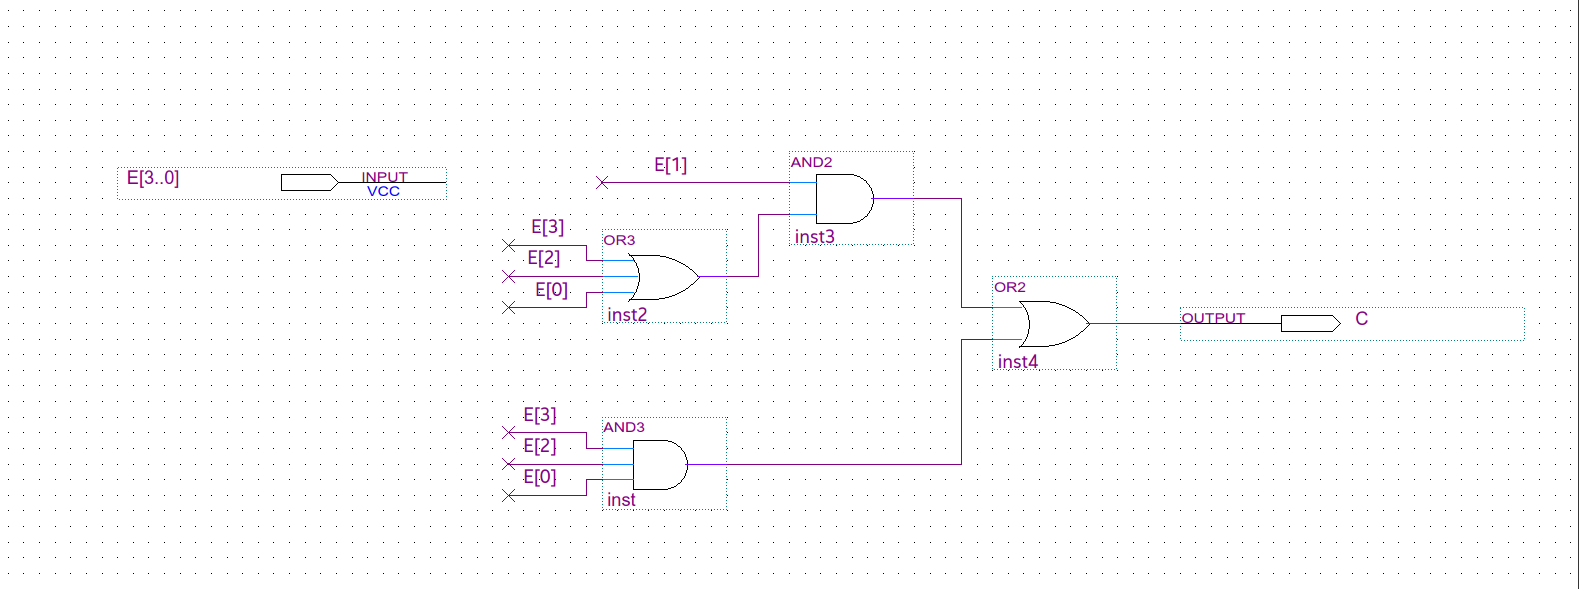
\includegraphics[width=\textwidth]{c_c}
  \caption{Implementación de $c(lamp)$ (Sección C)}
  \label{fig:c_c}
\end{figure}
\begin{figure}[H]
  \centering
  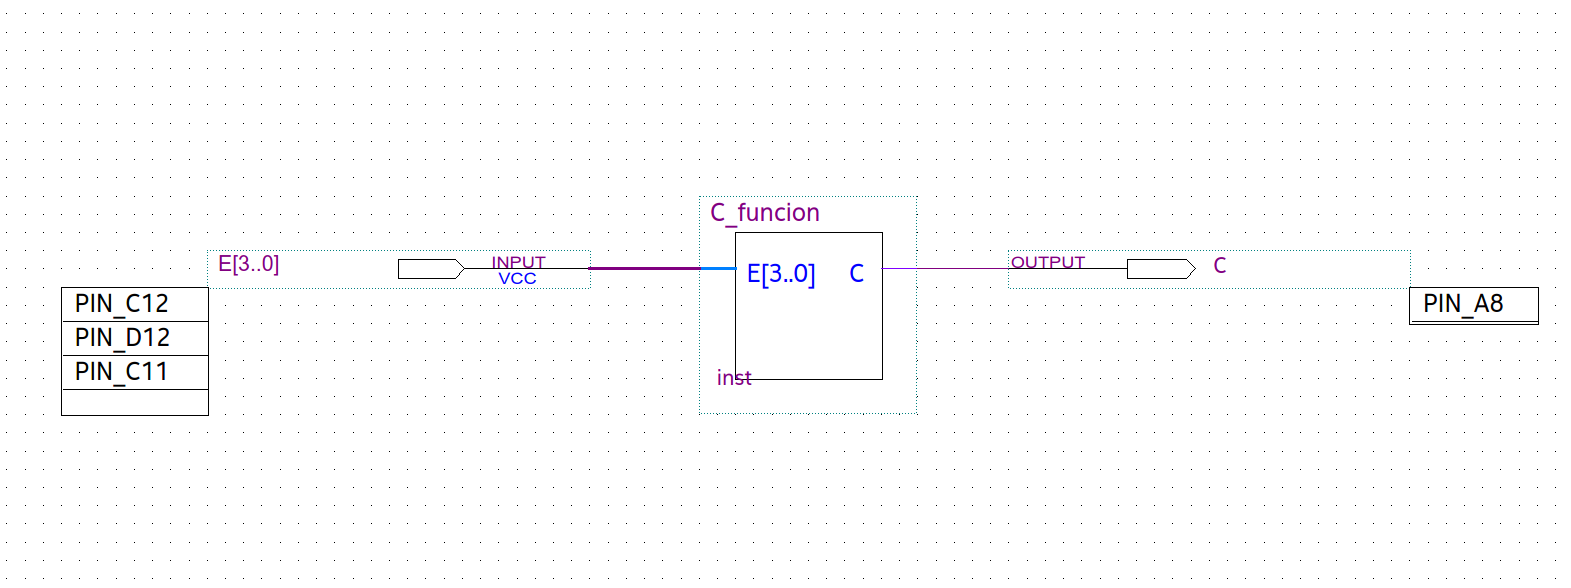
\includegraphics[width=\textwidth]{c_complete}
  \caption{Implementación completa (Sección C)}
  \label{fig:c_complete}
\end{figure}

Con lo anterior, y haciendo uso de un archivo \textit{University Program VWF}, 
se obtuvo el siguiente cronograma.
\begin{figure}[H]
  \centering
  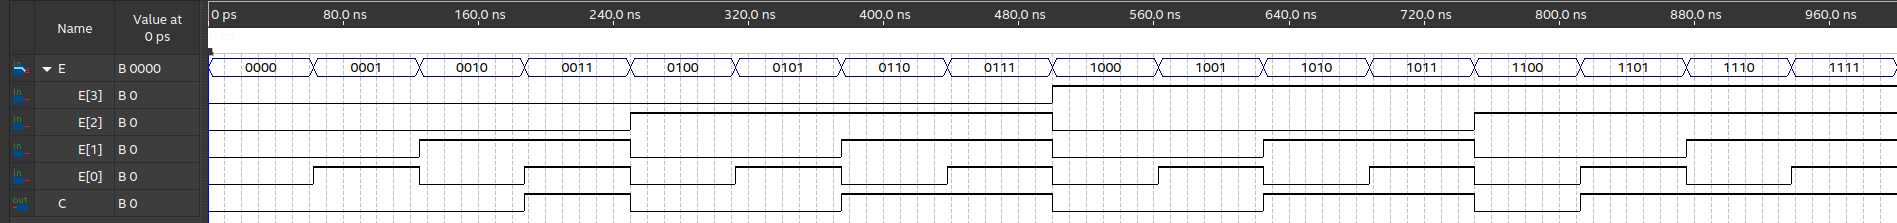
\includegraphics[width=\textwidth]{c_sim}
  \caption{Simulación del sistema (Sección C)}
  \label{fig:c_sim}
\end{figure}

\subsection{Ejecución en la FPGA}
Para poder cargar el programa en la tarjeta de desarrollo, fue importante 
investigar los pines para tomar las entradas y mostrar las salidas 
correctamente. Los pines utilizados se muestran en la Figura 
\ref{fig:c_complete}. Para las entradas, se utilizaron los pines: PIN\_C12, 
PIN\_D12, PIN\_C11 y PIN\_C10 (del bit más significativo al menos 
significativo, respectivamente). Por otro lado, para las salidas se ocuparon 
los pines: PIN\_A10, PIN\_A9 y PIN\_A8 (del bit más significativo al menos 
significativo, respectivamente).

Algunos casos de prueba se muestran a continuación.
\begin{figure}[H]
  \centering
  \begin{subfigure}[b]{0.45\textwidth}
    \centering
    \caption{Caso de prueba 1100 (12)}
    \label{fig:c_tarj_1}
    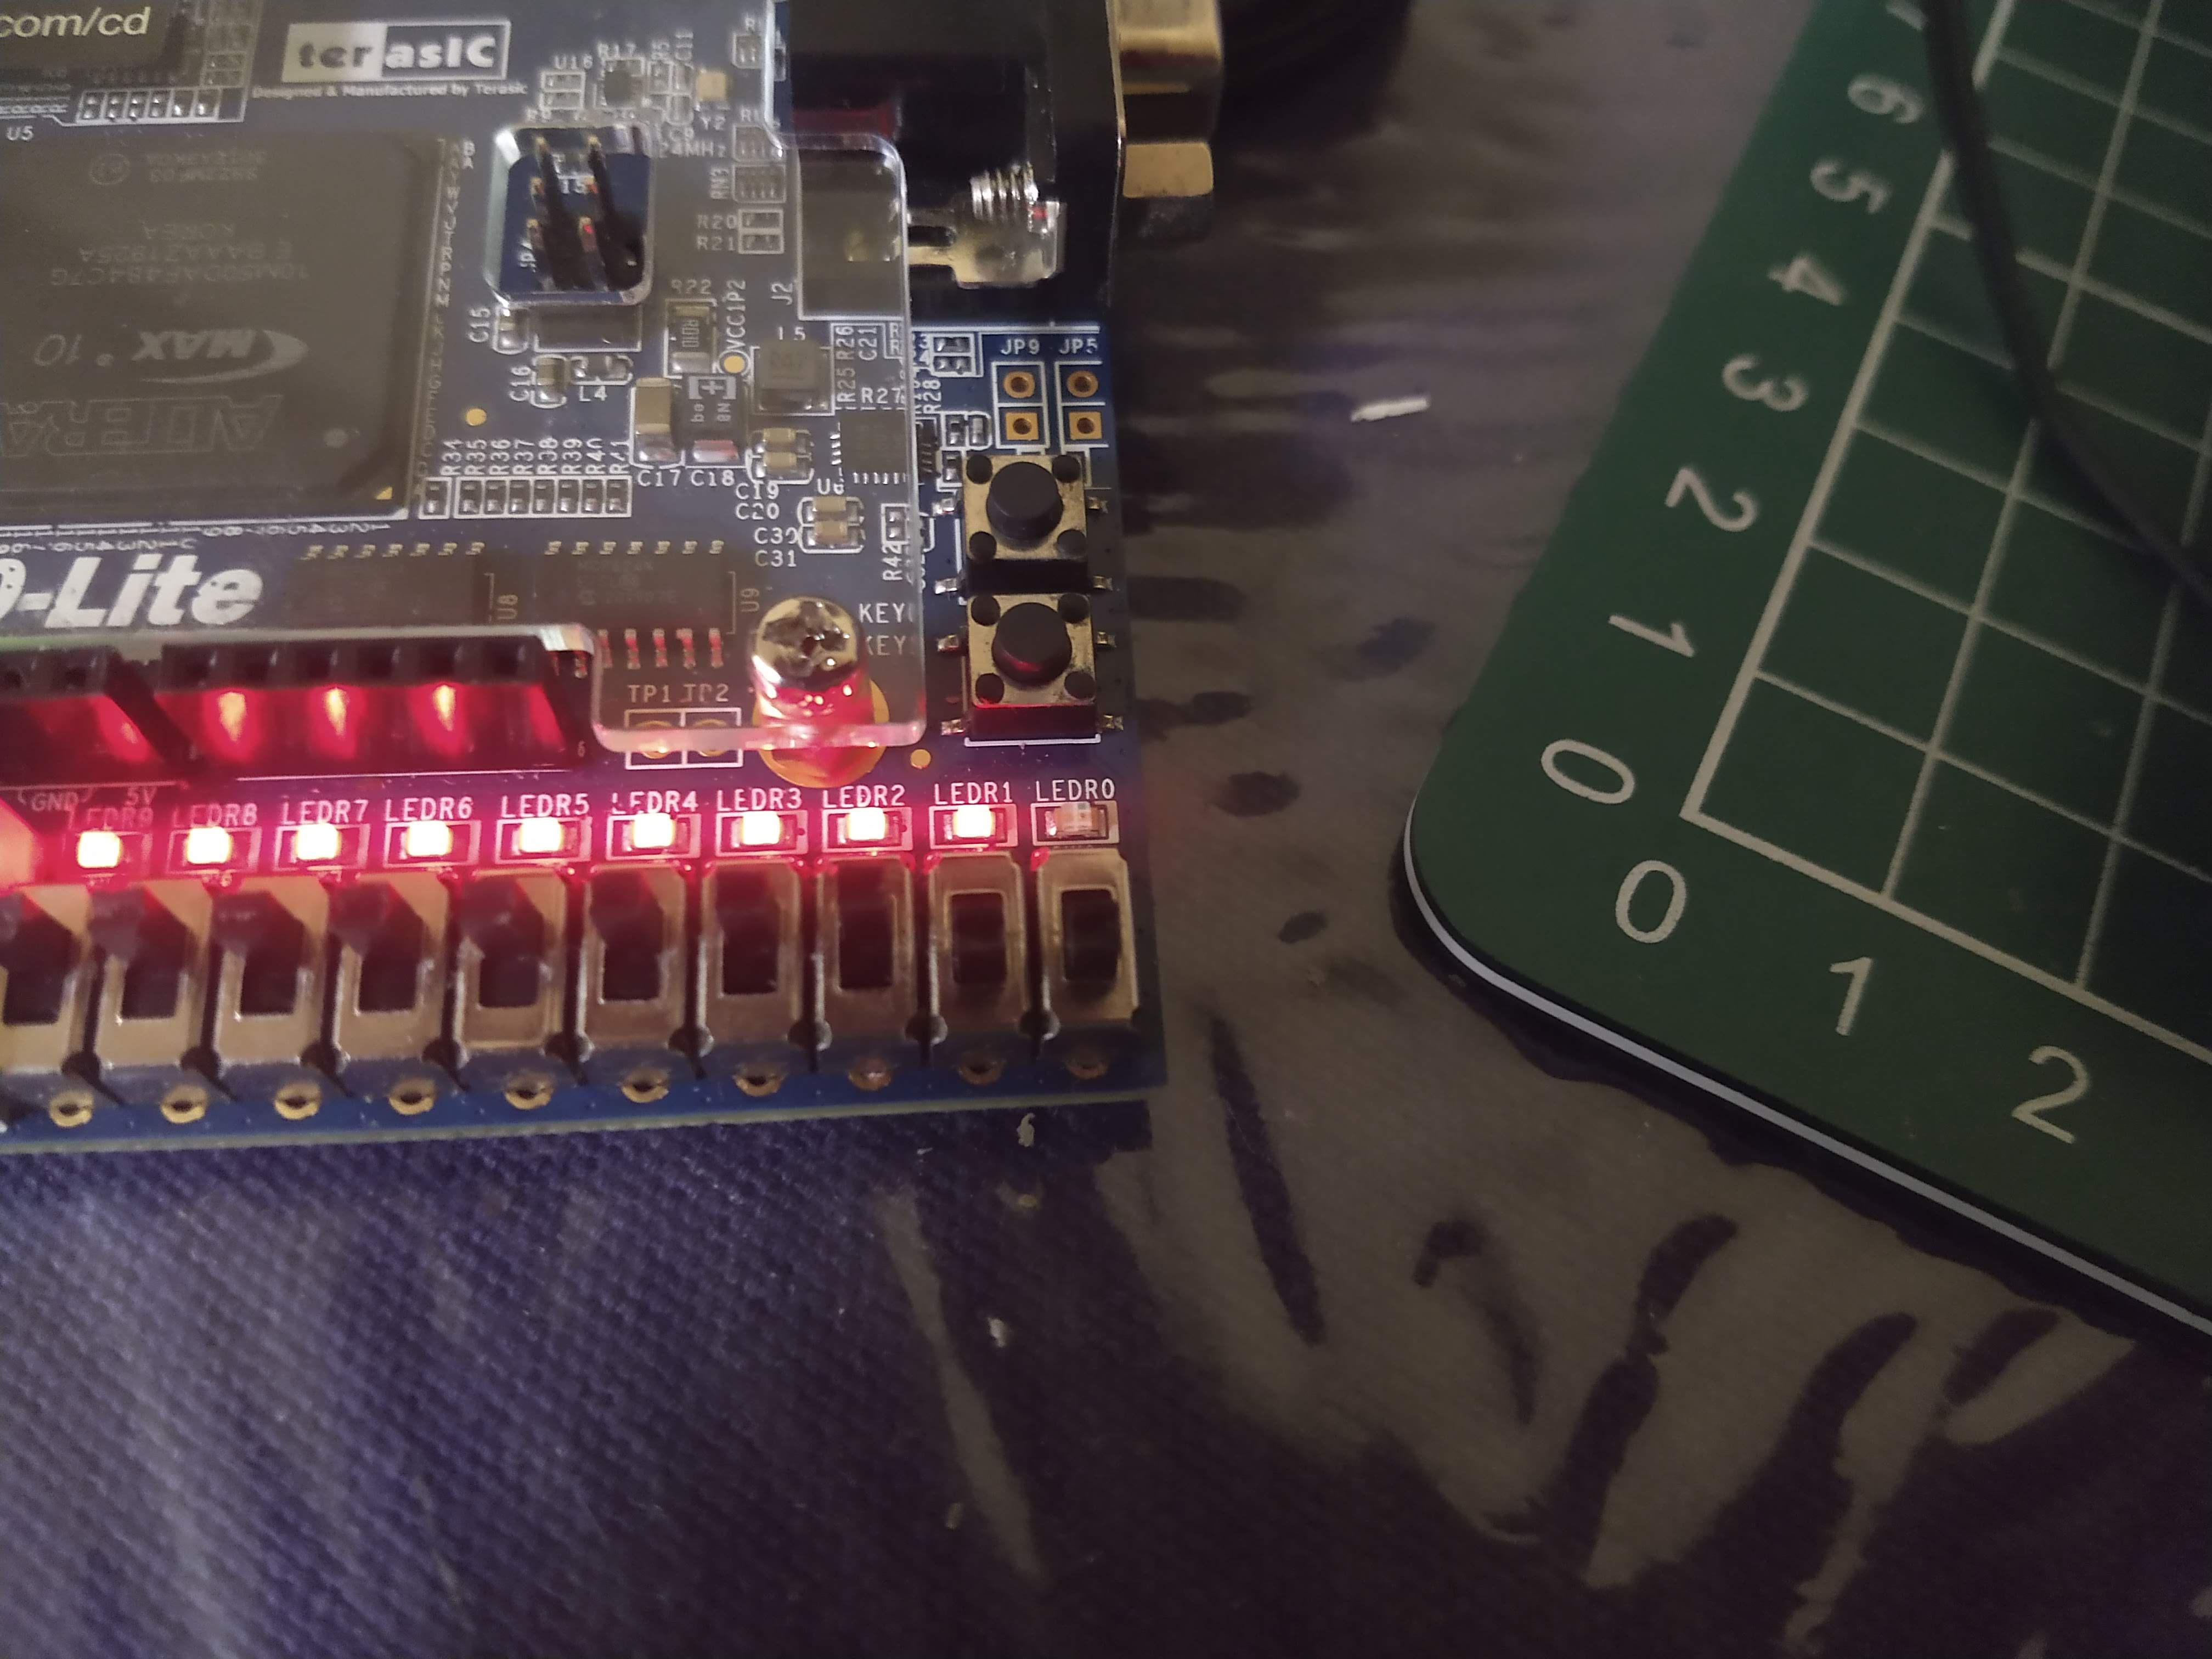
\includegraphics[width=\textwidth]{c_tarj_1}
  \end{subfigure}
  \begin{subfigure}[b]{0.45\textwidth}
    \centering
    \caption{Caso de prueba 1110 (14)}
    \label{fig:c_tarj_2}
    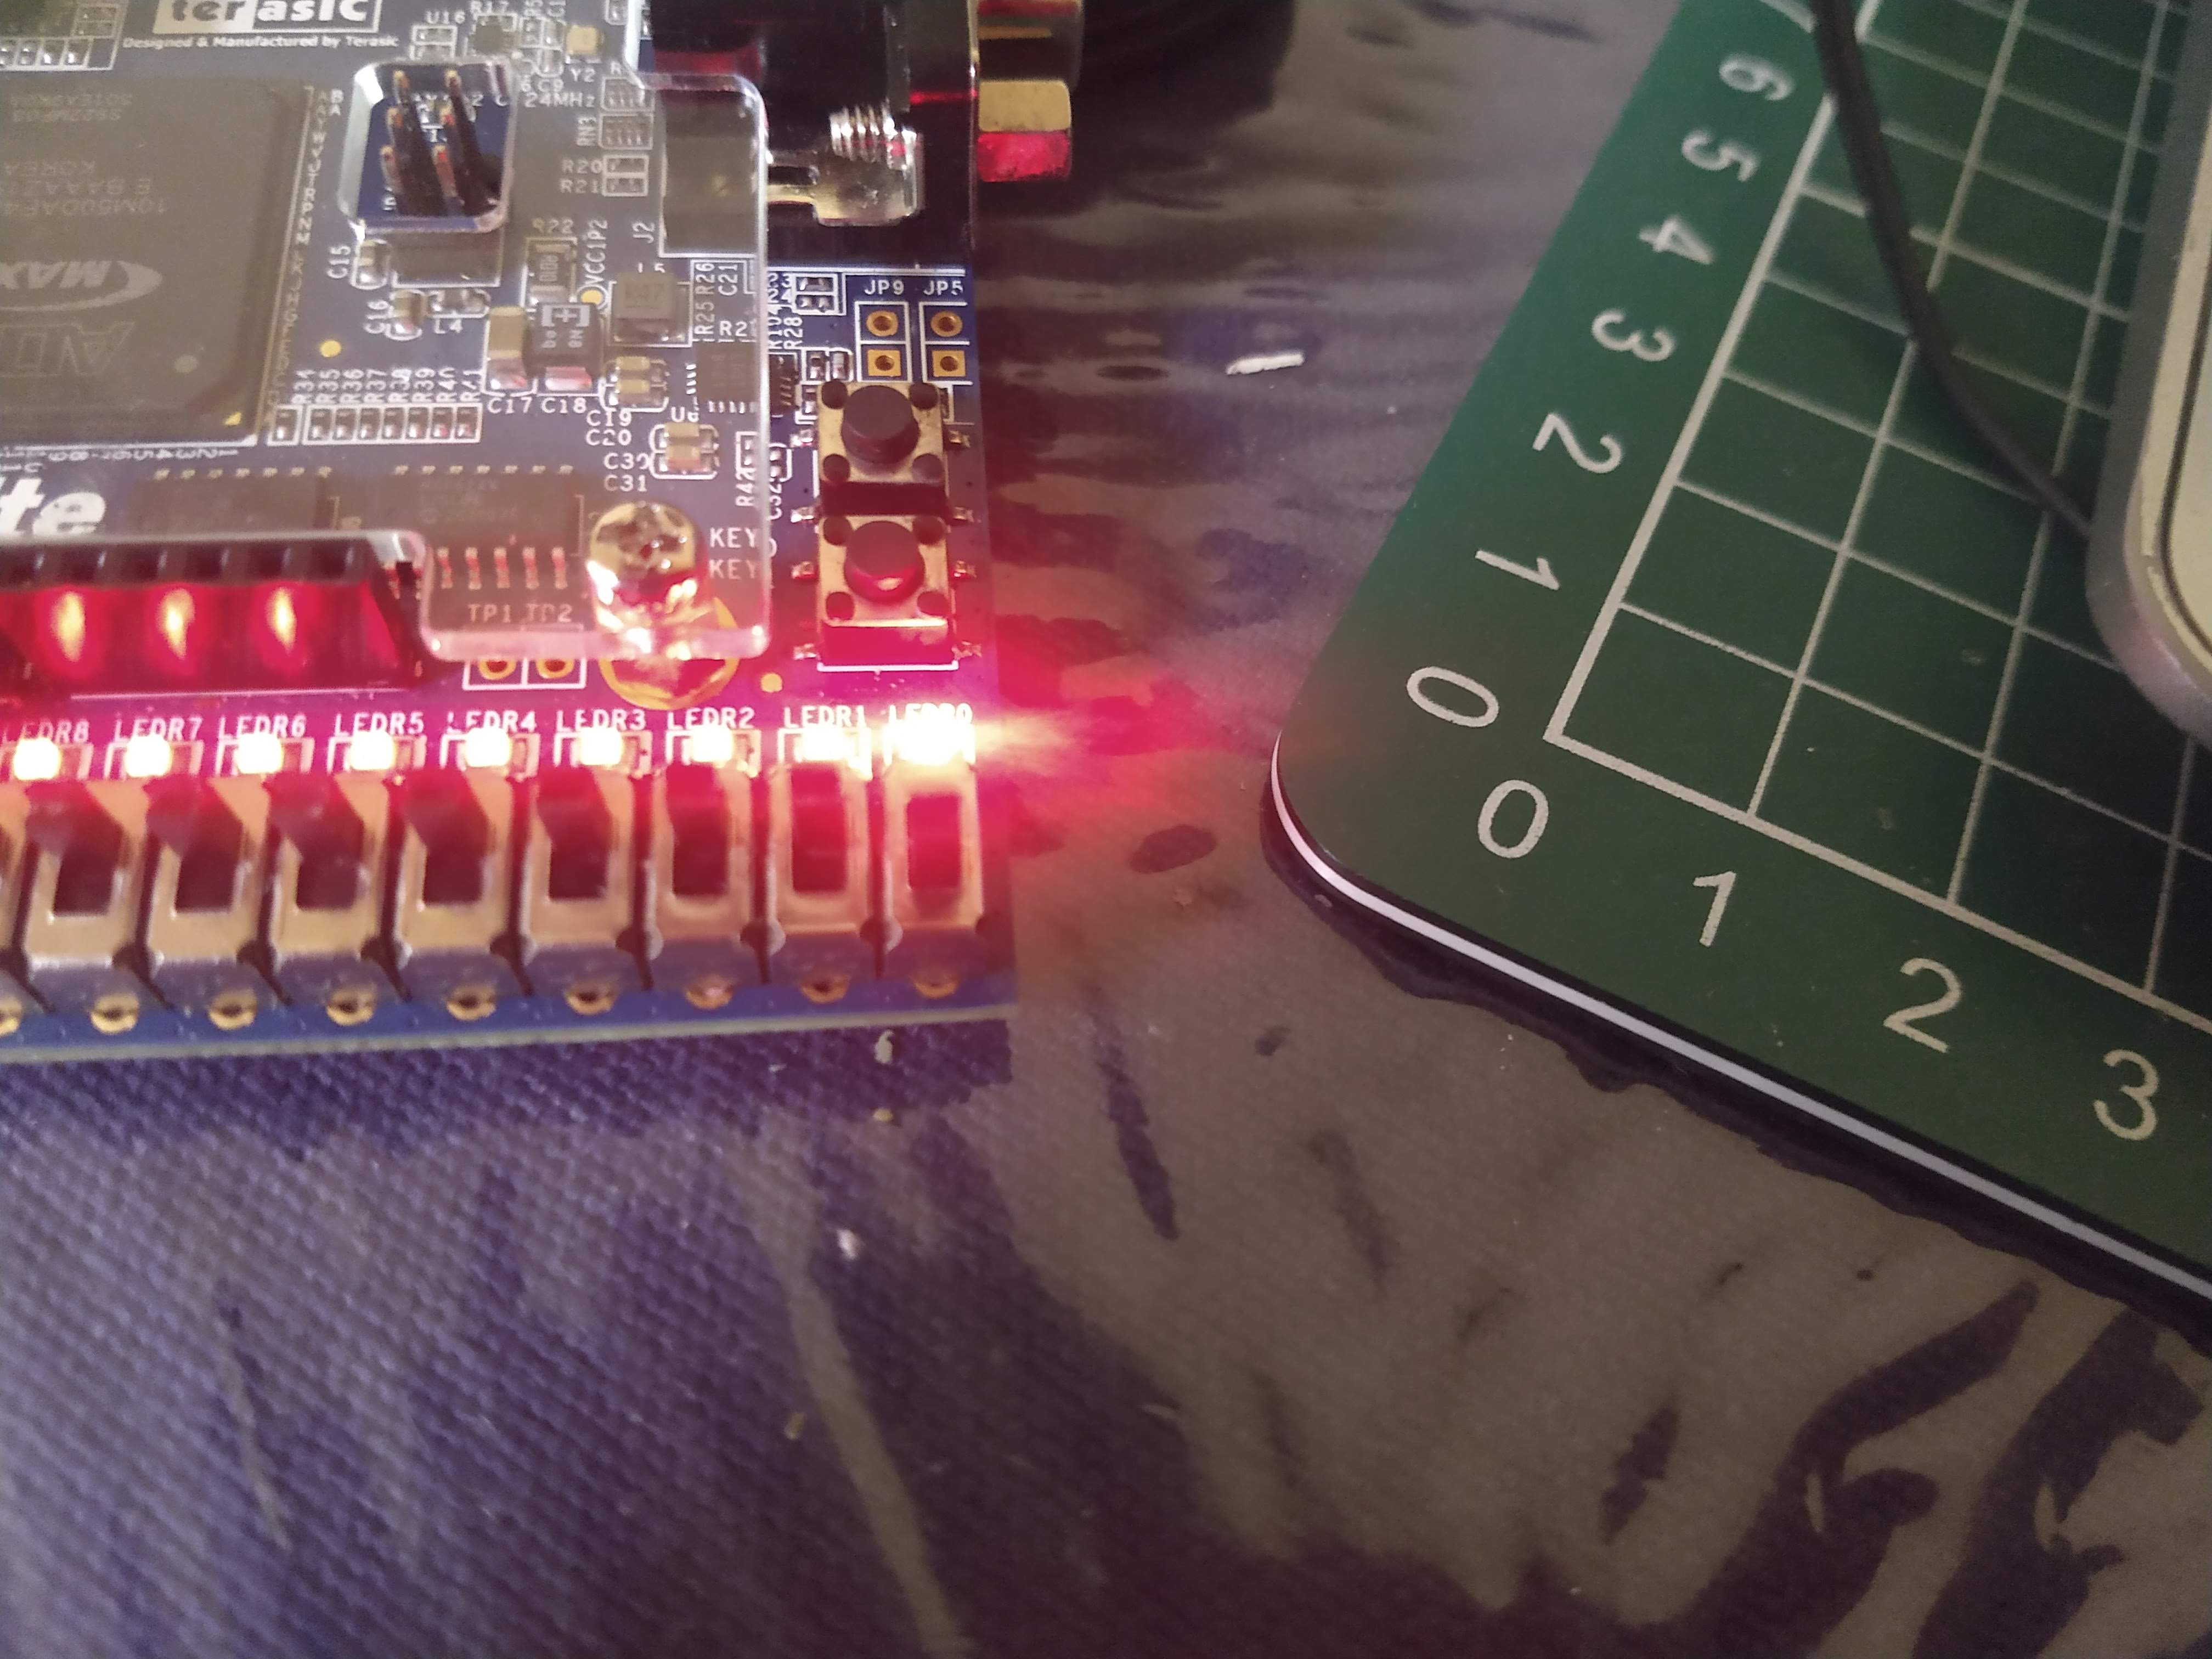
\includegraphics[width=\textwidth]{c_tarj_2}
  \end{subfigure}
  \begin{subfigure}[b]{0.45\textwidth}
    \centering
    \caption{Caso de prueba 1000 (15)}
    \label{fig:c_tarj_3}
    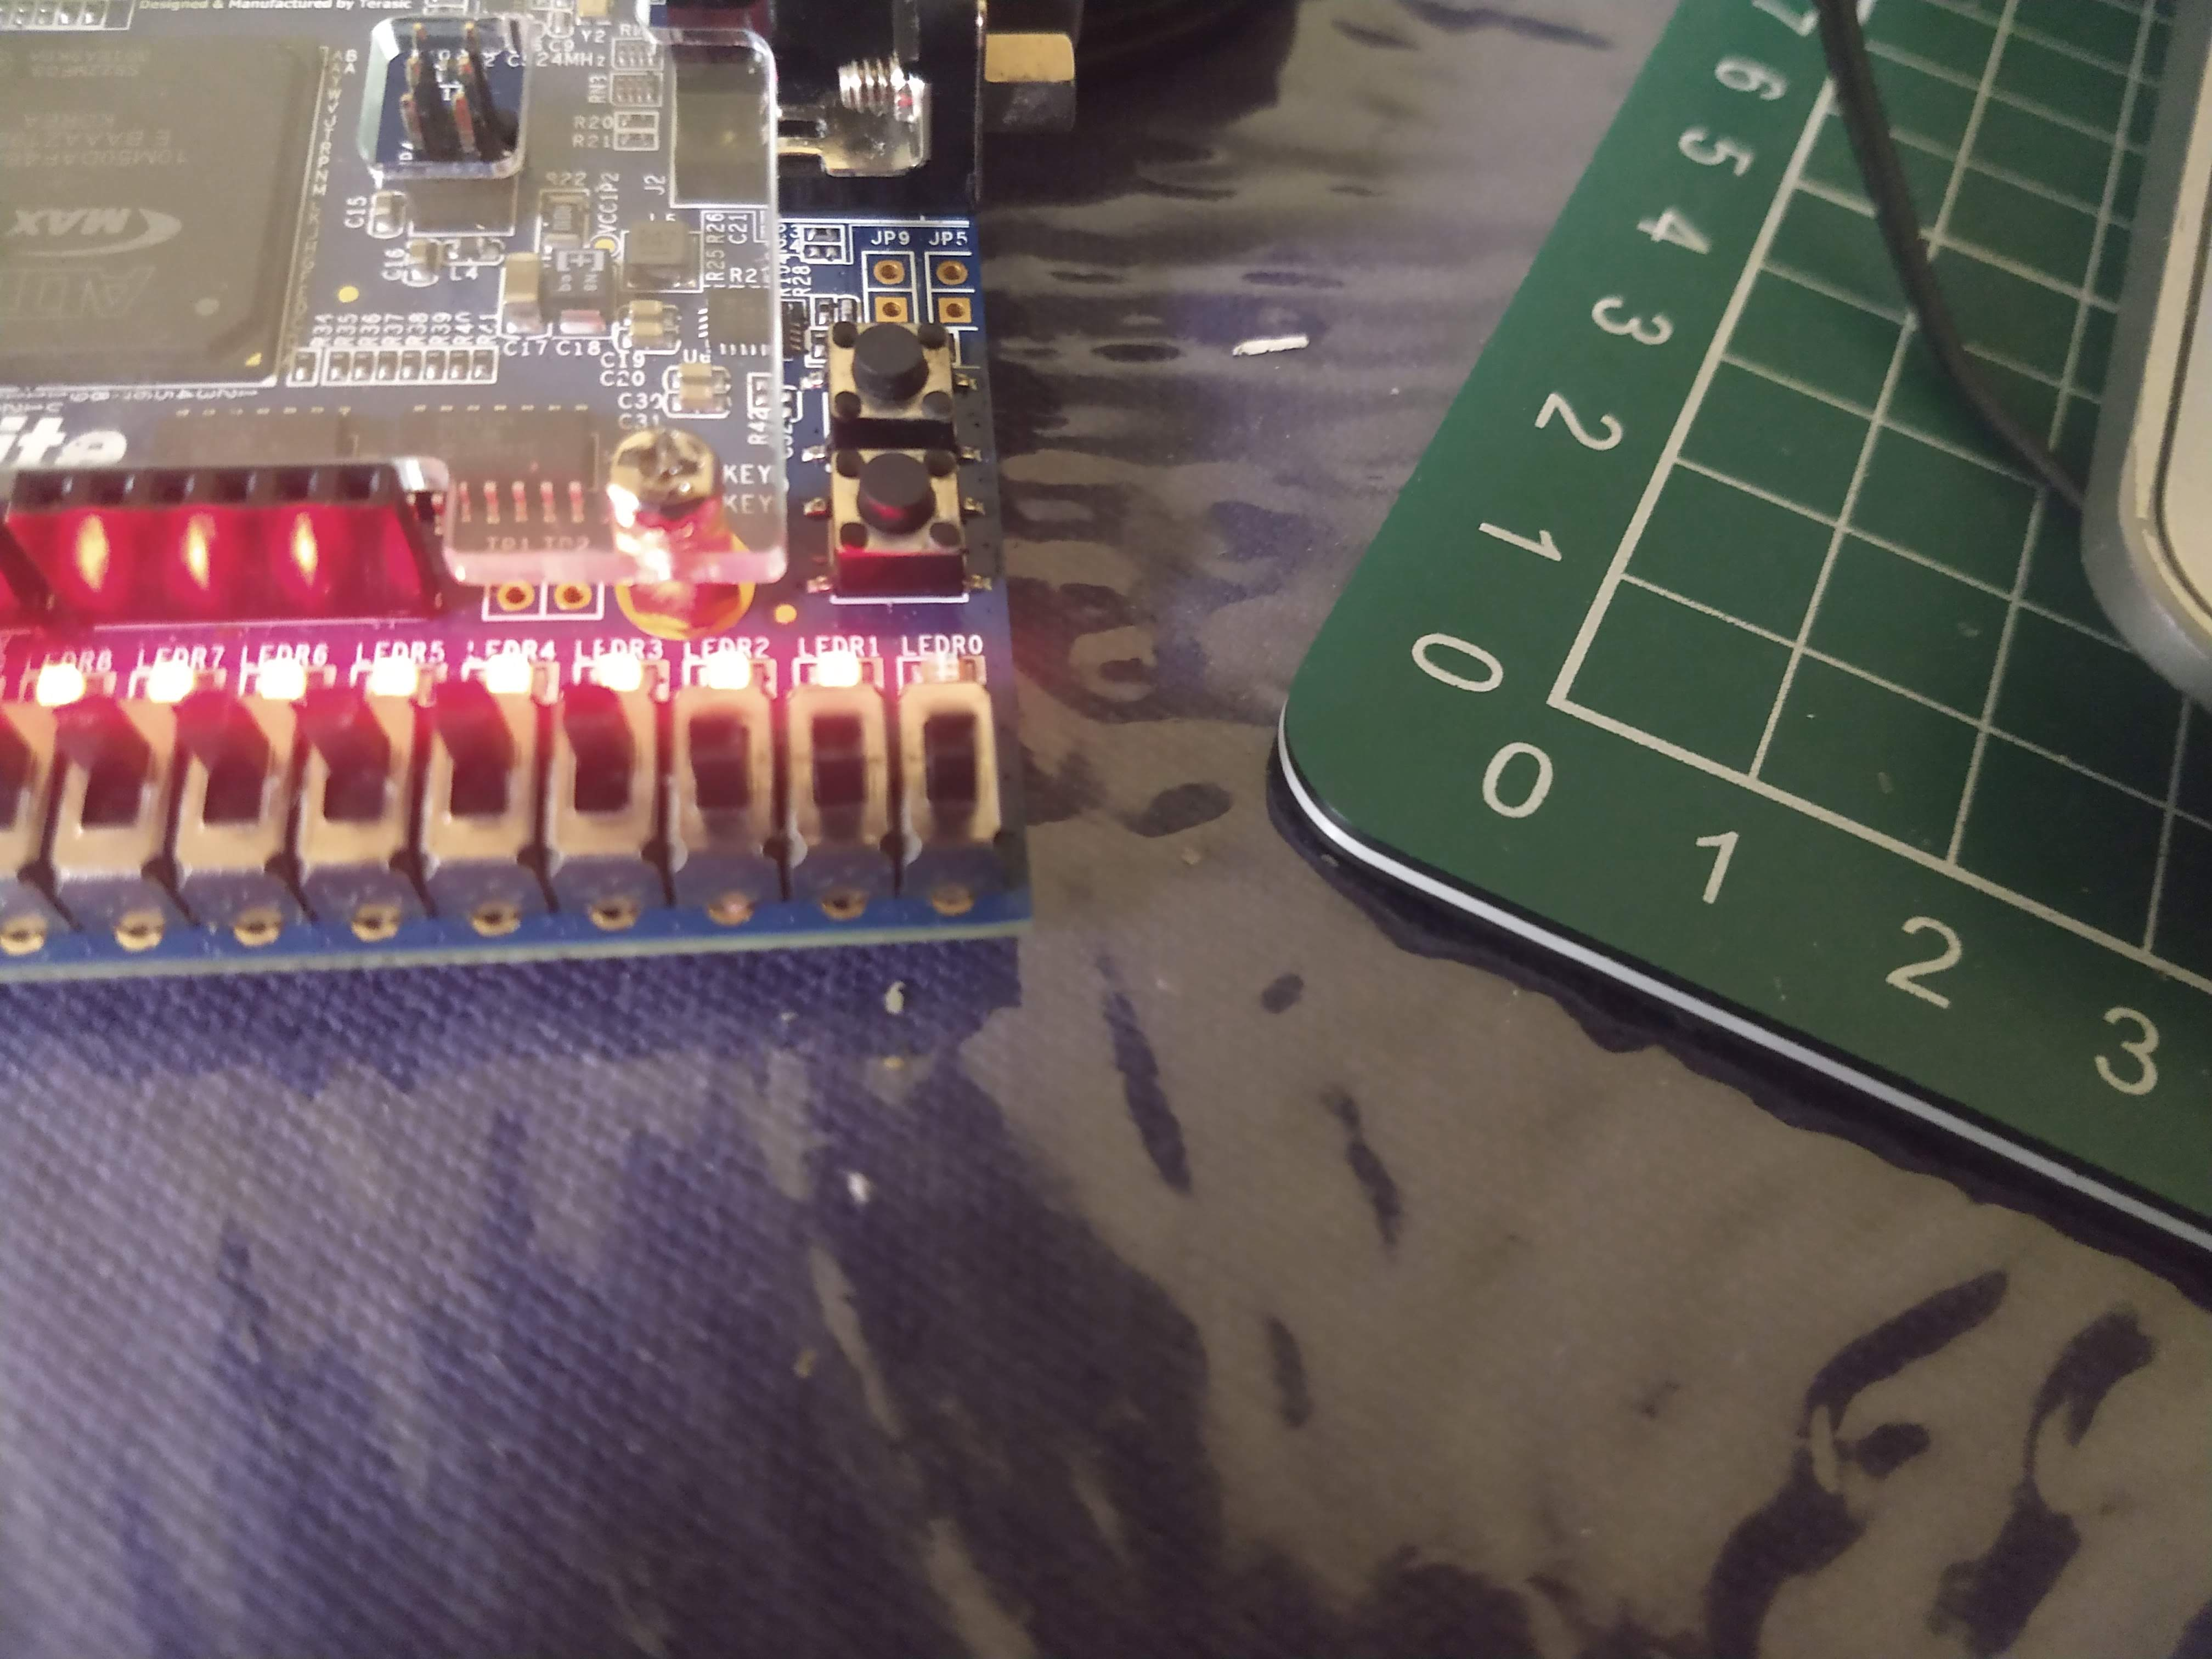
\includegraphics[width=\textwidth]{c_tarj_3}
  \end{subfigure}
  \begin{subfigure}[b]{0.45\textwidth}
    \centering
    \caption{Caso de prueba 1101 (13)}
    \label{fig:c_tarj_4}
    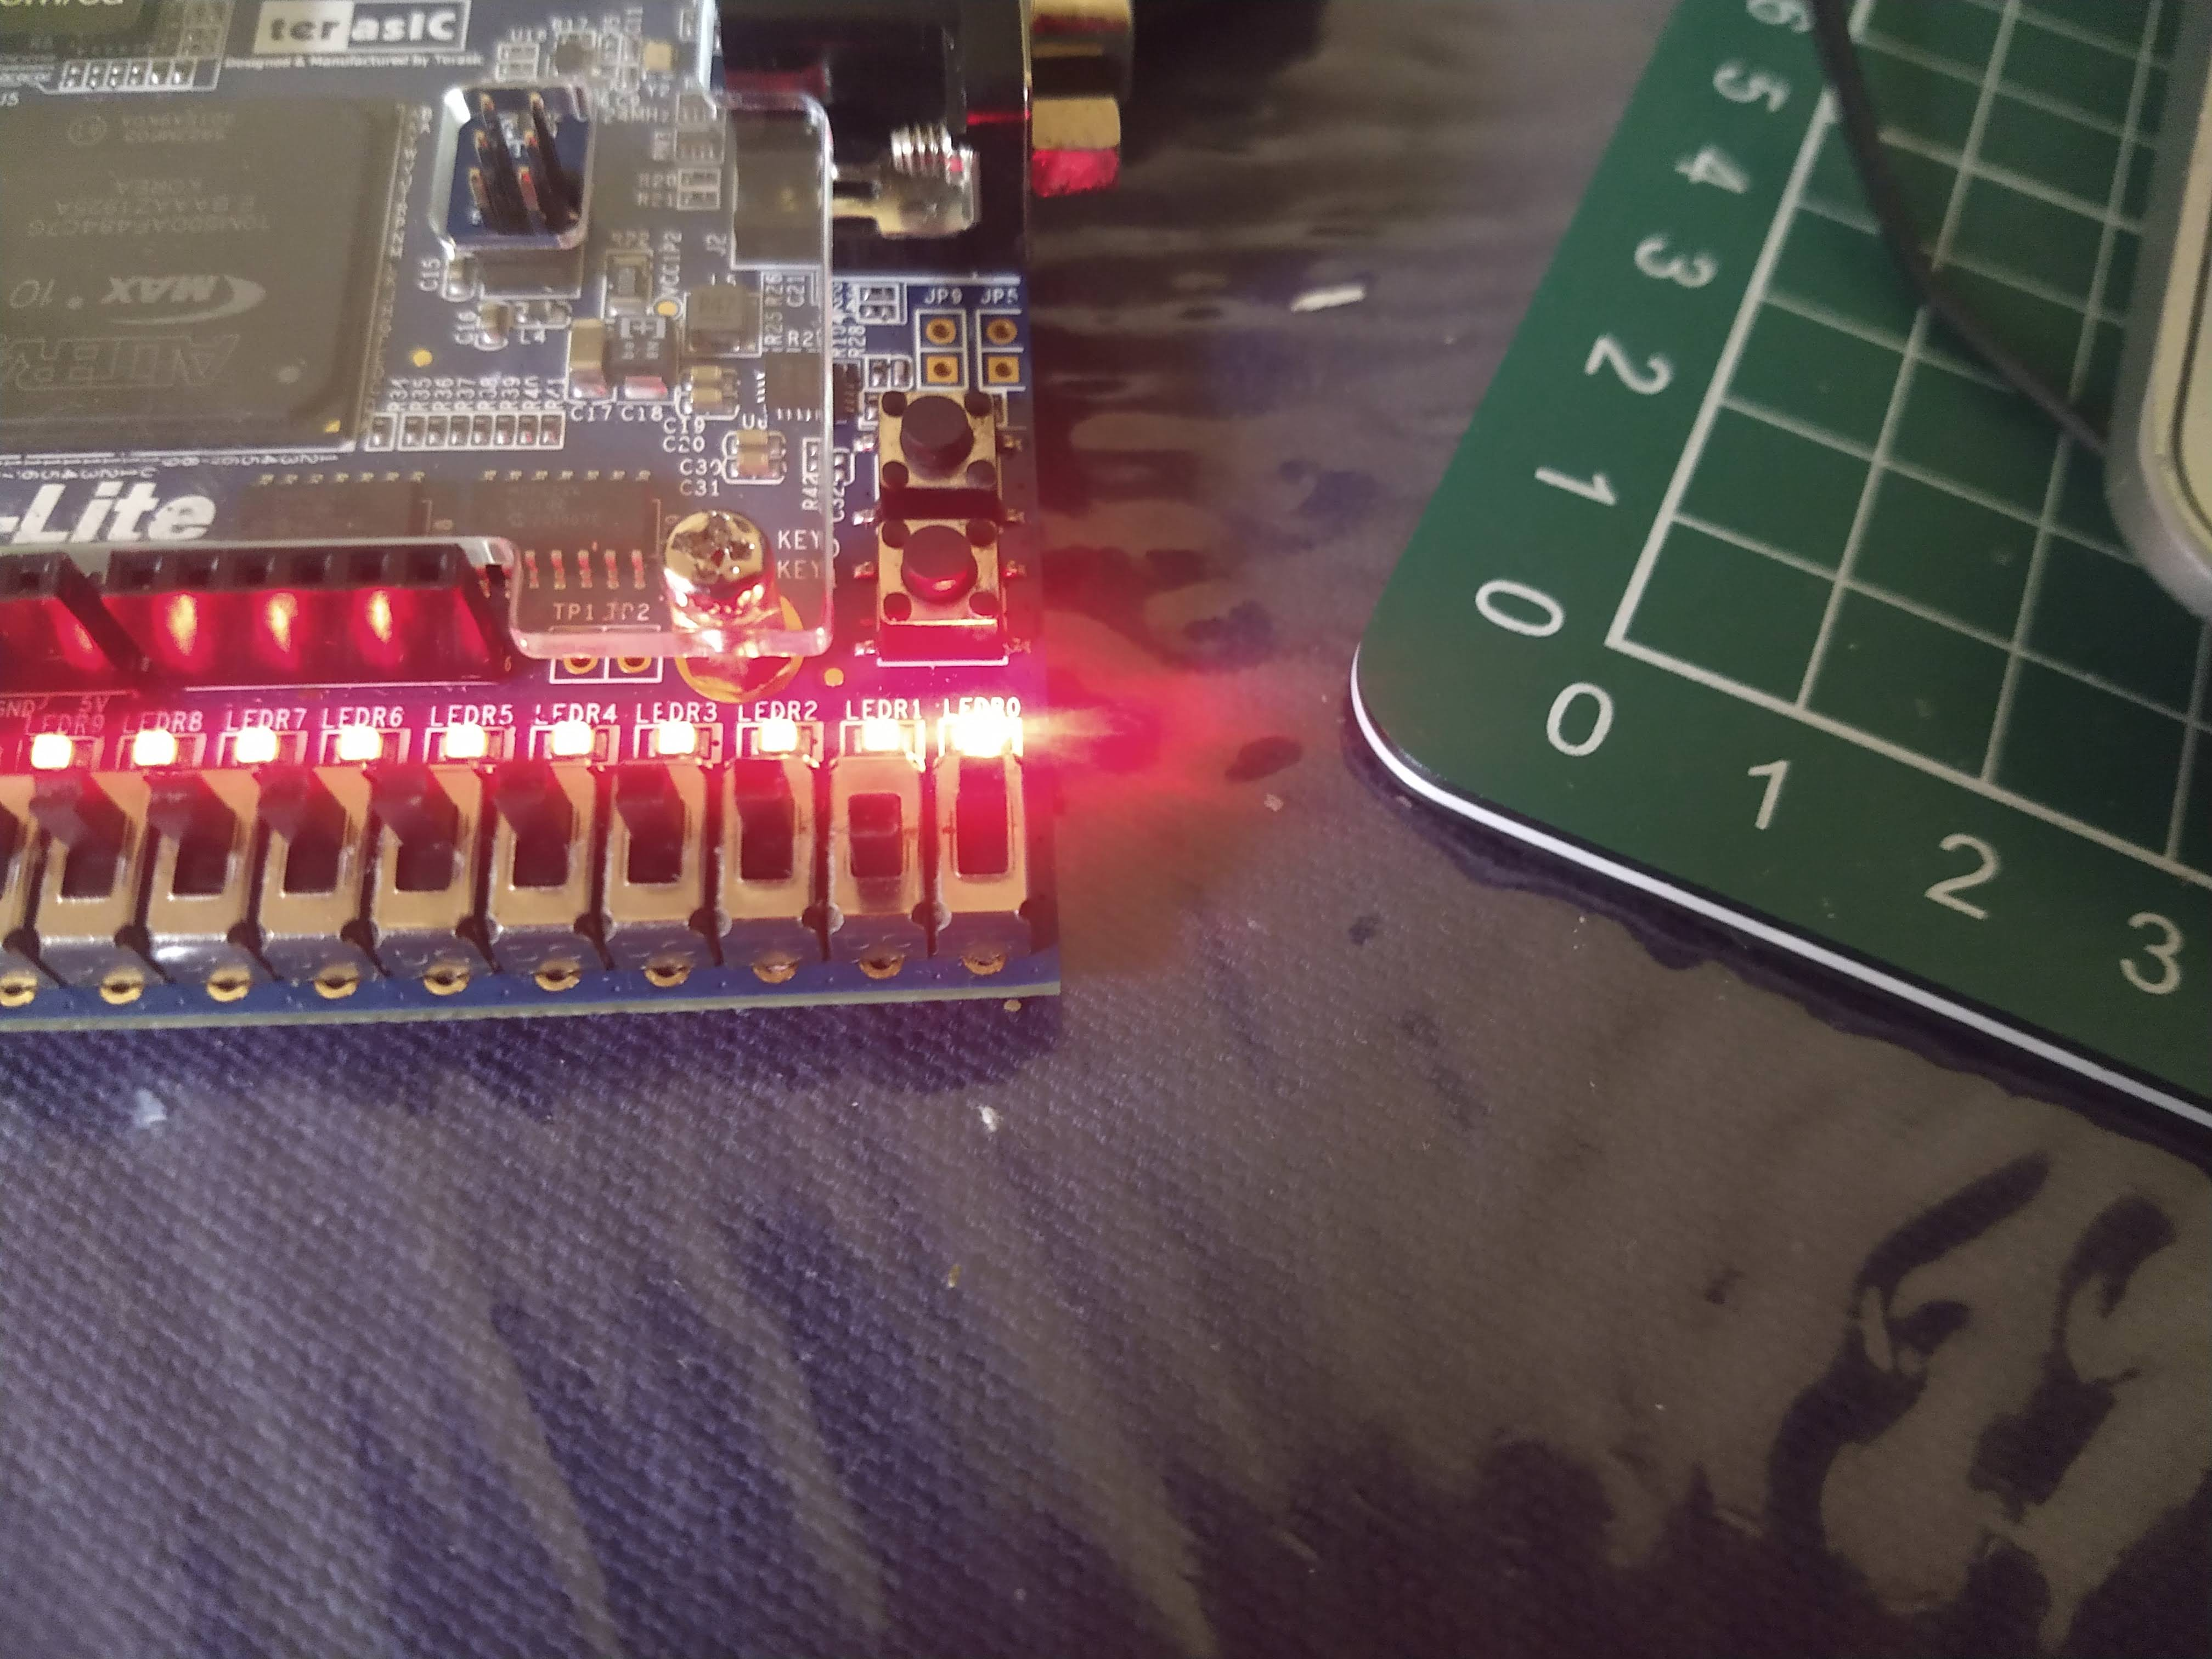
\includegraphics[width=\textwidth]{c_tarj_4}
  \end{subfigure}
  \caption{Casos de prueba (Sección A)}
\end{figure}

Los casos de prueba se comportan según lo esperado:
\begin{itemize}
  \item Para el caso de \ref{fig:c_tarj_1}: Luis y Ana quieren ir, pero Papá y 
  Mamá no. Hay un empate, entonces como la Mamá no quiere ir, no van.
  \item Para el caso de \ref{fig:c_tarj_2}: Luis, Ana y su Mamá quieren ir al 
    cine, como son mayoría, sí van.
  \item Para el caso de \ref{fig:c_tarj_3}: Sólo Luis sí quiere ir al cine, 
    como la mayoría no quiere ir, entonces no van.
  \item Para el caso de \ref{fig:c_tarj_4}: Todos quieren ir al cine, menos la 
    mamá, entonces sí van al cine porque gana la mayoría.
\end{itemize}
\end{document}

